\FloatBarrier
\section{Robustness}\label{app:robustness}
% Budget: 1 page.

\begin{table}[ht]
\centering\scriptsize
\caption{Robustness: mean total connectedness (\%) by method, share of DY connectedness lost once the common factor is removed (FNETS), and FNETS common-variance share.}
\label{tab:robustness}
\resizebox{\linewidth}{!}{\input{\tablepath/robustness_summary.tex}}
\end{table}

\begin{table}[ht]
\centering\scriptsize
\caption{Static connectedness: one estimate on the whole period (full sample) and on the subsamples before and after 2020. These are single long-sample estimates, not averages over rolling windows, so they differ from Tables~\ref{tab:criteria} and~\ref{tab:robustness}.}
\label{tab:static}
\input{\tablepath/static_connectedness.tex}
\end{table}

\begin{figure}[ht]
\centering
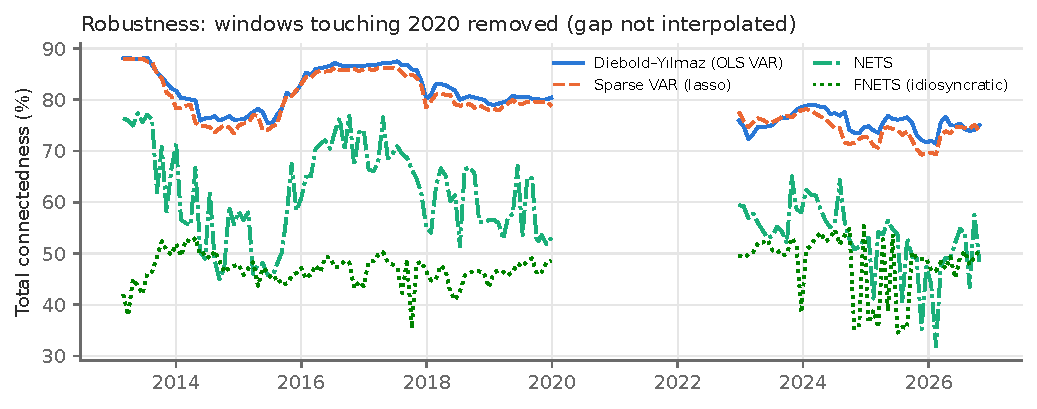
\includegraphics[width=\linewidth]{total_connectedness_ex2020}
\caption{Total connectedness excluding every window that contains a week of 2020.}
\label{fig:ex2020}
\end{figure}

Table~\ref{tab:robustness} reruns every method under alternative choices. The levels of Diebold--Yilmaz and lasso connectedness hardly move: between 79.7\% and 81.2\% and between 78.6\% and 80.5\% across all scenarios. NETS is the most sensitive to the window length (57.8\% with 78-week windows, 63.4\% with 130-week windows), as shorter windows leave the penalized estimator less information and make it keep fewer links. FNETS idiosyncratic connectedness ranges from 45.9\% to 50.5\%. The horizon matters very little: Diebold--Yilmaz changes by about 0.1 points between $H=2$ and $H=8$, and the sparse methods not at all, because their estimated lag coefficients are almost all zero and their variance decompositions are essentially driven by the contemporaneous covariance. Excluding the S\&P~500 lowers Diebold--Yilmaz connectedness by one point, and removing every window that contains a week of 2020 (141 windows left) lowers Diebold--Yilmaz, lasso and NETS connectedness by one to three points and leaves FNETS unchanged, without changing the ranking of the methods.

The main quantities are stable across scenarios. The share of Diebold--Yilmaz connectedness lost once the common factor is removed lies between 38\% (78-week windows) and 43\% (130-week windows), against 41\% in the baseline; the variance share of the common factor is 55--58\%. The ordering of the comparison criteria is also unchanged: the correlation of total connectedness with Diebold--Yilmaz is at least 0.96 for the lasso and between 0.84 and 0.90 for NETS, and in every scenario the dense estimators are the most stable from one window to the next, followed by NETS and then FNETS.

The subsample estimates in Table~\ref{tab:static} show a lower level of connectedness after 2020 than before: Diebold--Yilmaz connectedness falls from 83.0\% in 2011--2019 to 73.5\% in 2021--2026, and NETS from 69.6\% to 56.0\%. Idiosyncratic FNETS connectedness rises slightly (from 34.1\% to 39.6\%), while the variance share of the common factor falls from 58\% to 47\%. The decline after 2020 is therefore consistent with a weaker common component rather than with fewer idiosyncratic links. Figure~\ref{fig:ex2020} shows that, outside the windows that contain 2020, the time pattern of each method is the same as in the baseline.
